\chapter{Diseño}
\label{cap:diseno}

En este capítulo se va a hablar sobre el diseño del proyecto, así como de la arquitectura, herramientas y técnicas elegidas para el desarrollo del mismo.\\

El diseño es el desarrollo de aplicar una serie de métodos, técnicas y principios de diseño para traducir el modelo del análisis a una representación la cual sea posible ser codificada.\\

\section{Metodología}

La metodología seguida puede considerarse como \textit{Scrum}.\\

Al comienzo de este proyecto se tuvieron varias reuniones para establecer los objetivos y requisitos que debía de cumplir este proyecto, aunque no en demasiada profundidad, siendo esto una tarea que se llevo a cabo según lo establecido en el capítulo anterior.\\

Una vez finalizadas dichas reuniones iniciales, se establecieron una serie de fechas en las cuales se tuvieron otras reuniones para comprobar el estado del proyecto. Estas fechas coinciden con la planificación. Para cada reunión, se establecía una serie de objetivos que se debían alcanzar para el correcto desarrollo del proyecto y garantizar que se cumplía con la planificación establecida. De esta manera, se intercambiaron opiniones sobre la situación del proyecto, comentando posibles mejoras y solucionando las dudas surgidas durante las distintas etapas del desarrollo.\\

\section{Arquitectura}

El estilo arquitectónico utilizado para la realización de este proyecto ha sido el modelo vista controlador, ya que se adapta correctamente a las necesidades del sistema.
Los elementos de una arquitectura MVC son:

\begin{itemize}
\item Modelo: Es el encargado del conocimiento del dominio de la aplicación.
\item Vista: Responsable de mostrar las diferentes características del modelo al usuario.
\item Controlador: Elemento que responde a la interacción del usuario, realizando las peticiones necesarias al modelo y la vista.
\end{itemize}

Una vez definido el estilo arquitectónico se va a pasar a hablar de las herramientas que se han usado.

\section{Herramientas usadas}

En esta sección vamos a comentar las herramientas que han sido usadas durante la realización del proyecto.

\subsection{Android Studio}

Aunque no es estrictamente necesario para desarrollar aplicaciones Android, es posible utilizar eclipse por ejemplo, he decidido usarlo ya que es muy sencillo de entender y facilita al programador muchas tareas. Esto ha sido muy importante ya que, como he comentado antes, mi experiencia con Android era muy reducida.\\

Android Studio es el entorno de desarrollo integrado, \textit{IDE}, oficial para la plataforma Android. Por esta razón la documentación es abundante, lo que supone un gran punto a su favor.\\

\begin{figure}[H] %con el [H] le obligamos a situar aquí la figura
\centering
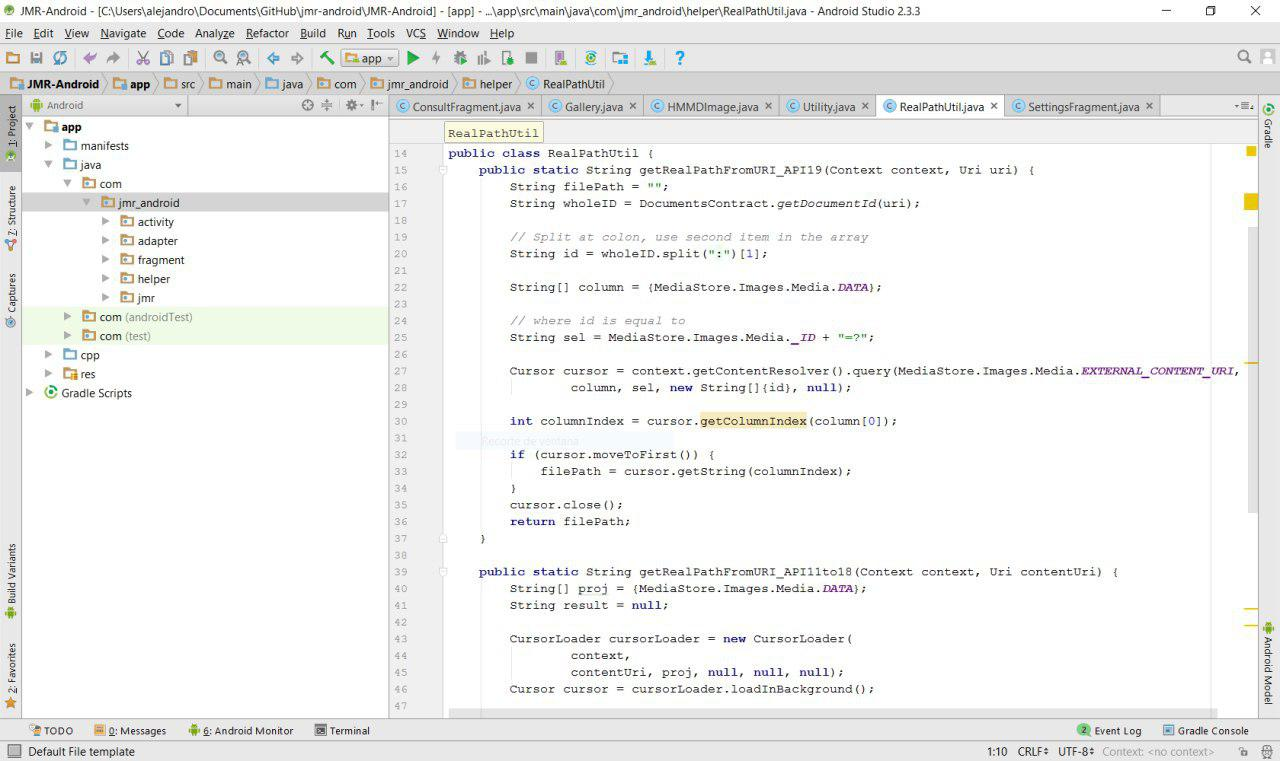
\includegraphics[scale=0.5]{imagenes/android-studio.jpg}  %el parámetro scale permite agrandar o achicar la imagen. En el nombre de archivo puede especificar directorios
\label{android-studio.jpg}
\caption{Ejemplo de proyecto Android Studio}
\end{figure}

Otra de las cosas interesantes de este \textit{IDE} es la posibilidad de diseñar interfaces de una manera muy sencilla e intuitiva, permitiendo arrastrar los elementos a las posiciones deseadas. Por lo que no se requiere un gran nivel de programación para estas tareas. Aunque si hay que comentar, que si se necesita hacer cosas más complicadas, o que no sean las estándar, si es necesario un nivel de programación avanzado, ya que en dicho caso, la ayuda proporcionada por Android Studio para estas tareas se reduce.\\ 

\subsection{Git y GitHub}

Al tratarse de un proyecto de esta magnitud, ha sido necesario utilizar una herramienta de control de versiones, como es natural se ha utilizado git.\\

También se ha usado GitHub, que se trata de un lugar donde alojar nuestros proyectos utilizando el sistema de control de versiones Git. Por lo tanto, podemos entender que git y GitHub van de la mano, al menos en este caso.\\

El repositorio del proyecto se puede consultar \href{https://github.com/acasadoquijada/jmr-android}{aquí}.

Para llevar un control del proyecto se han usado los elementos conocidos como \textit{Milestones} y \textit{Issues} por GitHub.\\

Podemos entender un \textit{Issue} como una tarea por realizar, siendo un ejemplo, \textit{seleccionar imagen de la galería}. Se les puede añadir información extra, como a que \textit{Milestone} está asociado, que persona es la encargada de solucionarlo, o se puede añadir una etiqueta para establecer el tipo.\\

\begin{figure}[H] %con el [H] le obligamos a situar aquí la figura
\centering
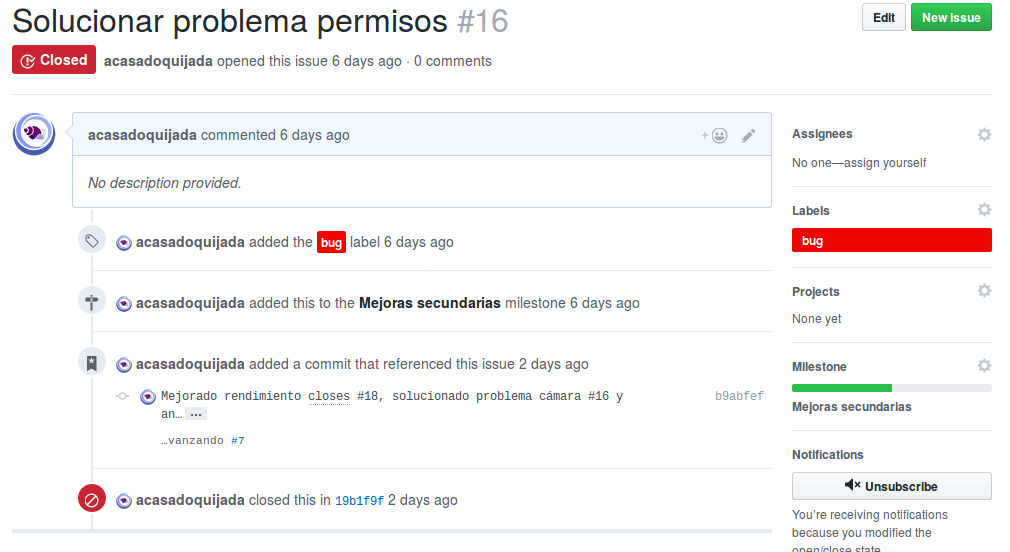
\includegraphics[scale=0.4]{imagenes/issue.png}  %el parámetro scale permite agrandar o achicar la imagen. En el nombre de archivo puede especificar directorios
\label{issue.png}
\caption{Ejemplo de issue}
\end{figure}

Por otro lado, se encuentran los \textit{Milestones}, que podemos considerarlos como hitos, es decir, un \textit{Milestone} está compuesto por varios \textit{Issues}. Por lo que también puede ser vistos como una agrupación de \textit{Issues}, una gran tarea dividida en pequeñas subtareas.\\

\begin{figure}[H] %con el [H] le obligamos a situar aquí la figura
\centering
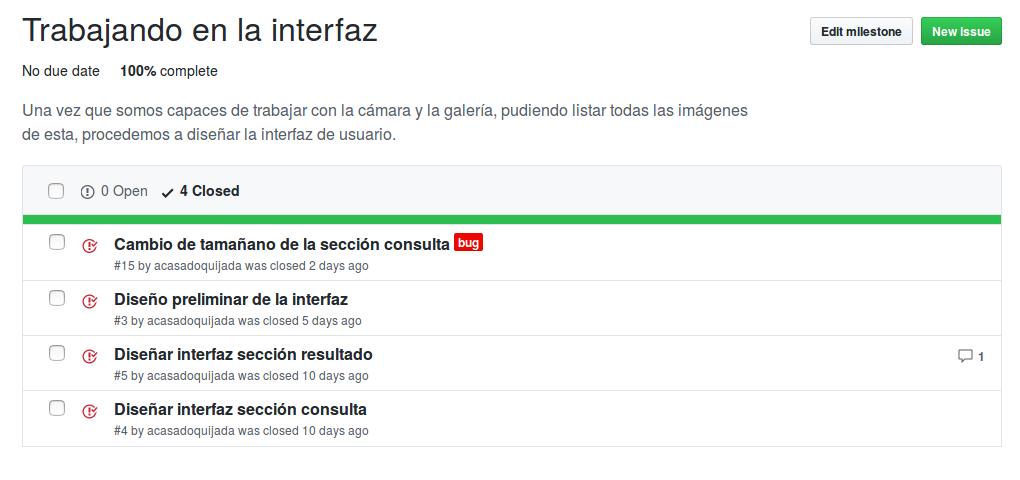
\includegraphics[scale=0.4]{imagenes/milestone.png}  %el parámetro scale permite agrandar o achicar la imagen. En el nombre de archivo puede especificar directorios
\label{milestone.png}
\caption{Ejemplo de milestone}
\end{figure}

Como se puede entender, usar ambos es de vital importancia si se desea llevar a cabo un proyecto de gran magnitud.

\subsection{Dispotivio de pruebas}

Aunque Android Studio nos ofrece la posibilidad de utilizar un emulador para lanzar la aplicación, he decidido utilizar mi dispositivo móvil, por motivos de eficiencia y comodidad. Debido a que no se podía comprobar de manera real algunos aspectos de la propia aplicación, como el consumo de memoria o el propio rendimiento de las consultas.\\

Mi smartphone es un \textit{Xiaomi redmi 4 pro}, y cuenta con las siguientes características destacables:

\begin{itemize}
\item CPU: Qualcomm Snapdragon 625, con ocho núcleos y 2GHz 
\item Memoria: 3 GB
\item Almacenamiento: 32 GB
\end{itemize}

Se tratan de unas características que suelen ser habituales de encontrar en los smartphones actuales, por lo que ha sido un gran sujeto de pruebas.

\section{Tecnicas}

Para programar en Android se utiliza \textit{Java} para la lógica, y \textit{XML} para las interfaces de usuario.\\

Como es habitual, el desarrollo en Java ha seguido un paradigma de programación orientada a objetos, \textit{POO}. En el que se han desarrollado una serie de clases que se han organizado en distintos paquetes. Esto será explicado posteriormente.\\ 

Comentar que se ha utilizado también \textit{Android NDK}. Se trata de un conjunto de herramientas que nos permiten implementar partes de la aplicación en código nativo, como \textit{C} o \textit{C++}. Esta opción es perfecta para usar en los cálculos que realiza la aplicación. Como en el caso anterior se comentará con más detalle en su correspondiente sección.\\

\begin{figure}[H] %con el [H] le obligamos a situar aquí la figura
\centering
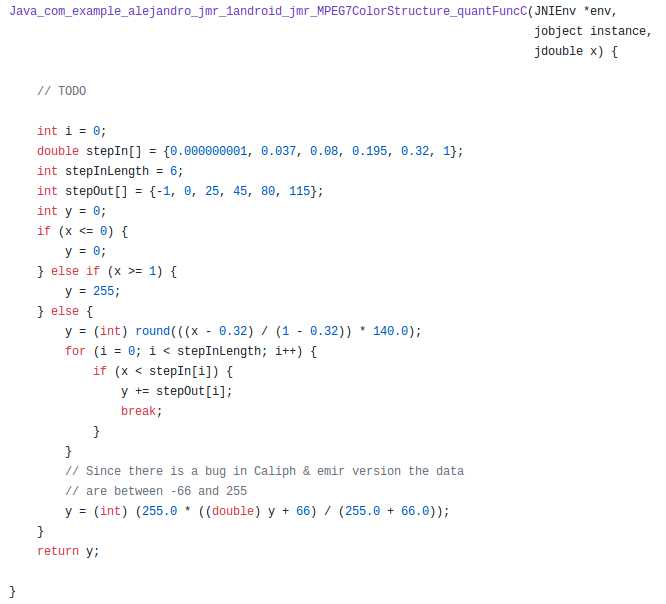
\includegraphics[scale=0.6]{imagenes/ndk.png}  %el parámetro scale permite agrandar o achicar la imagen. En el nombre de archivo puede especificar directorios
\label{ndk.png}
\caption{Ejemplo de código Android ndk}
\end{figure}

Por último comentar que se ha usado \textit{XML} para las interfaces de usuario, la mayor parte del tiempo apoyándose en el soporte proporcionado por Android Studio, pero que a la hora de realizar cosas mas complejas se ha tenido que escribir manualmente dicho código XML.

\begin{figure}[H] %con el [H] le obligamos a situar aquí la figura
\centering
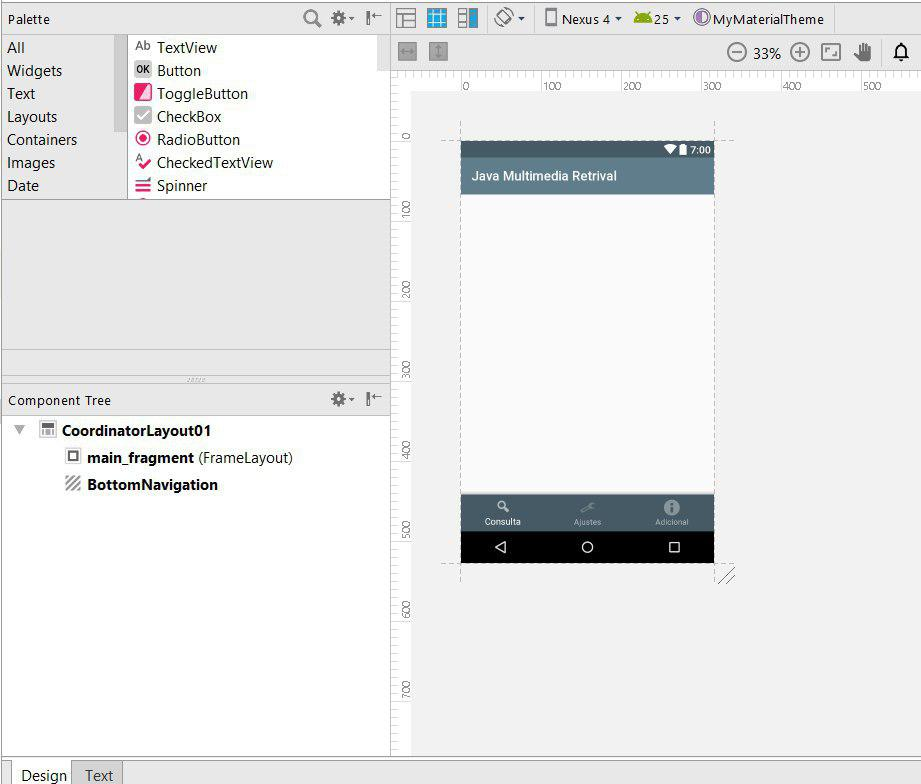
\includegraphics[scale=0.6]{imagenes/interfaz-android-studio.jpg}  %el parámetro scale permite agrandar o achicar la imagen. En el nombre de archivo puede especificar directorios
\label{interfaz-android-studio.jpg}
\caption{Ejemplo de proyecto Android Studio}
\end{figure}


\section{Diagrama de clases del diseño}

Tras todo lo anterior es hora de definir el diagrama de clases de diseño de este proyecto.\\

Esto describe de manera gráfica las características de las clases e interfaces software así de las relaciones entre ellas dentro de una aplicación. Es extremadamente importante realizar un buen diagrama de clases, ya que las clases representadas en él van a ser implementadas y si hubiese algún tipo de error podría hacer que el proyecto fuera inviable, teniendo que volver a diseñar el diagrama. Puede darse el caso de que observando el diagrama de clases, se note que el sistema carece de las funcionalidades deseadas.

\begin{landscape}

\begin{figure}[H] %con el [H] le obligamos a situar aquí la figura
\centering
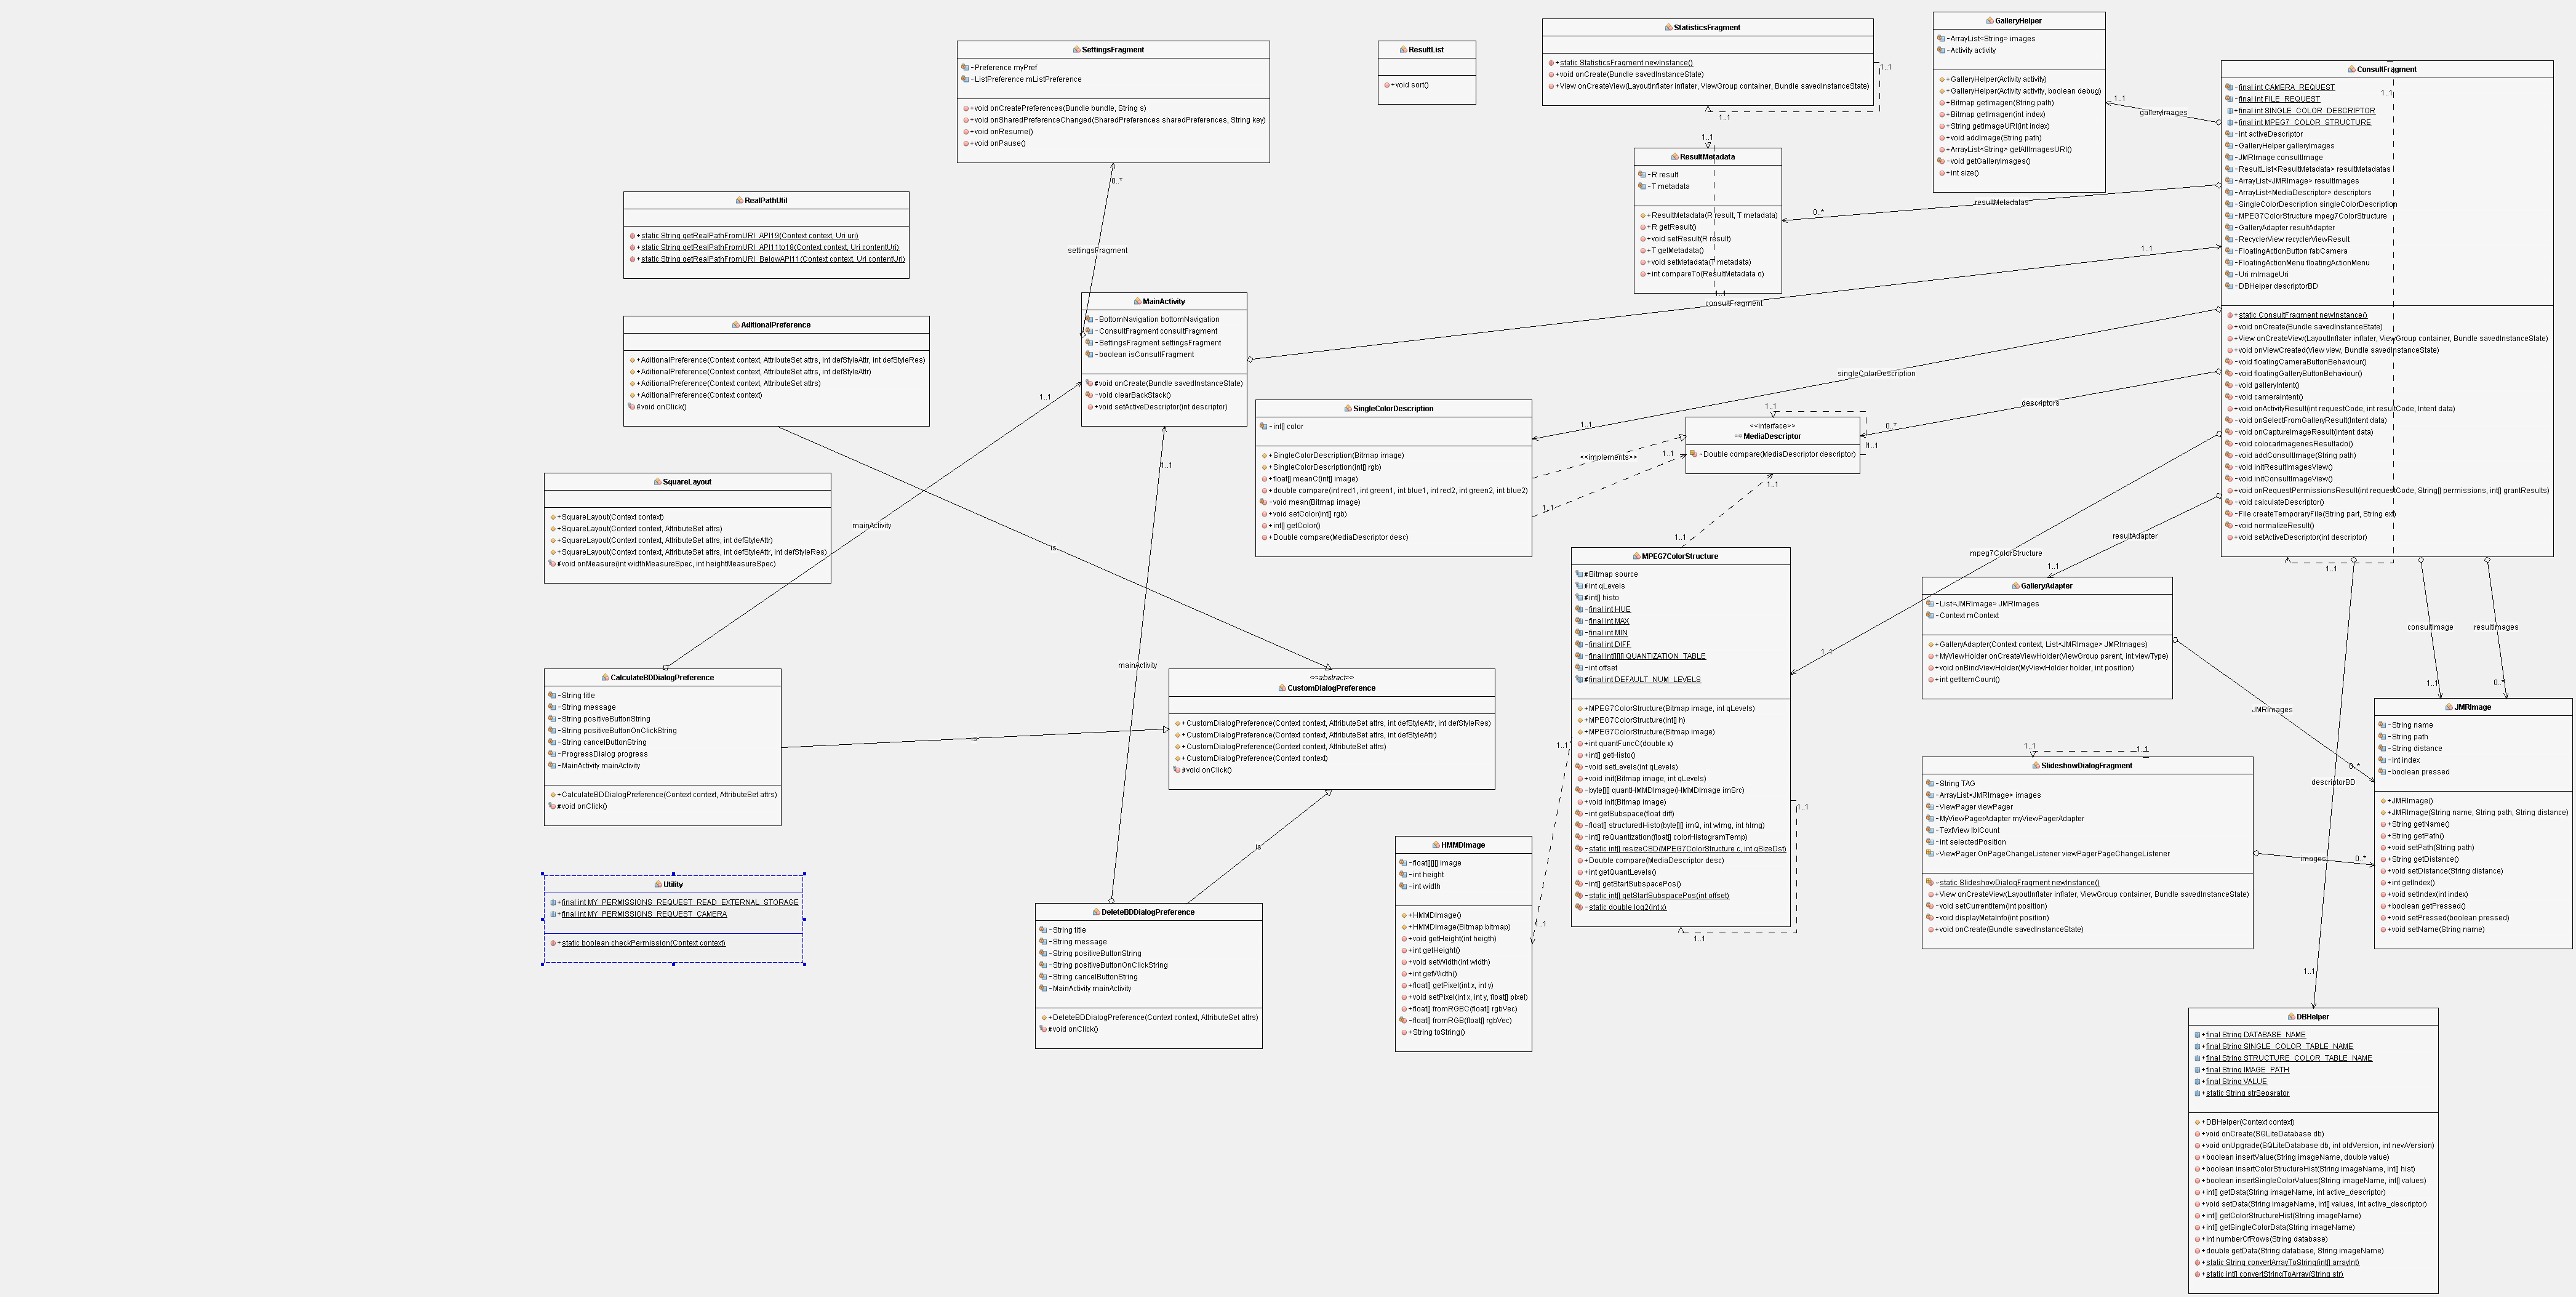
\includegraphics[scale=0.15, angle=270]{imagenes/diagramaTotal.png}  %el parámetro scale permite agrandar o achicar la imagen. En el nombre de archivo puede especificar directorios
\label{diagramaTotal.jpg}
\caption{Diagrama de clases del diseño}
\end{figure}




\end{landscape}













